\chapter{Design and Assembly of the UACS PCB}
\label{kap:design}

The UACS reader is a printed circuit board on which an STM32H523CET6 microcontroller, an
RFID front-end module, an I\textsuperscript{2}S audio amplifier, a micro-SD slot, a
CAN~FD transceiver, and associated connectors are assembled. User feedback is provided by
two dual-colour LEDs. The board can be powered either from a USB-C connector or from the
RJ45 CAN cable.

\begin{figure}[p]
  \centering
  \rotatebox{-90}{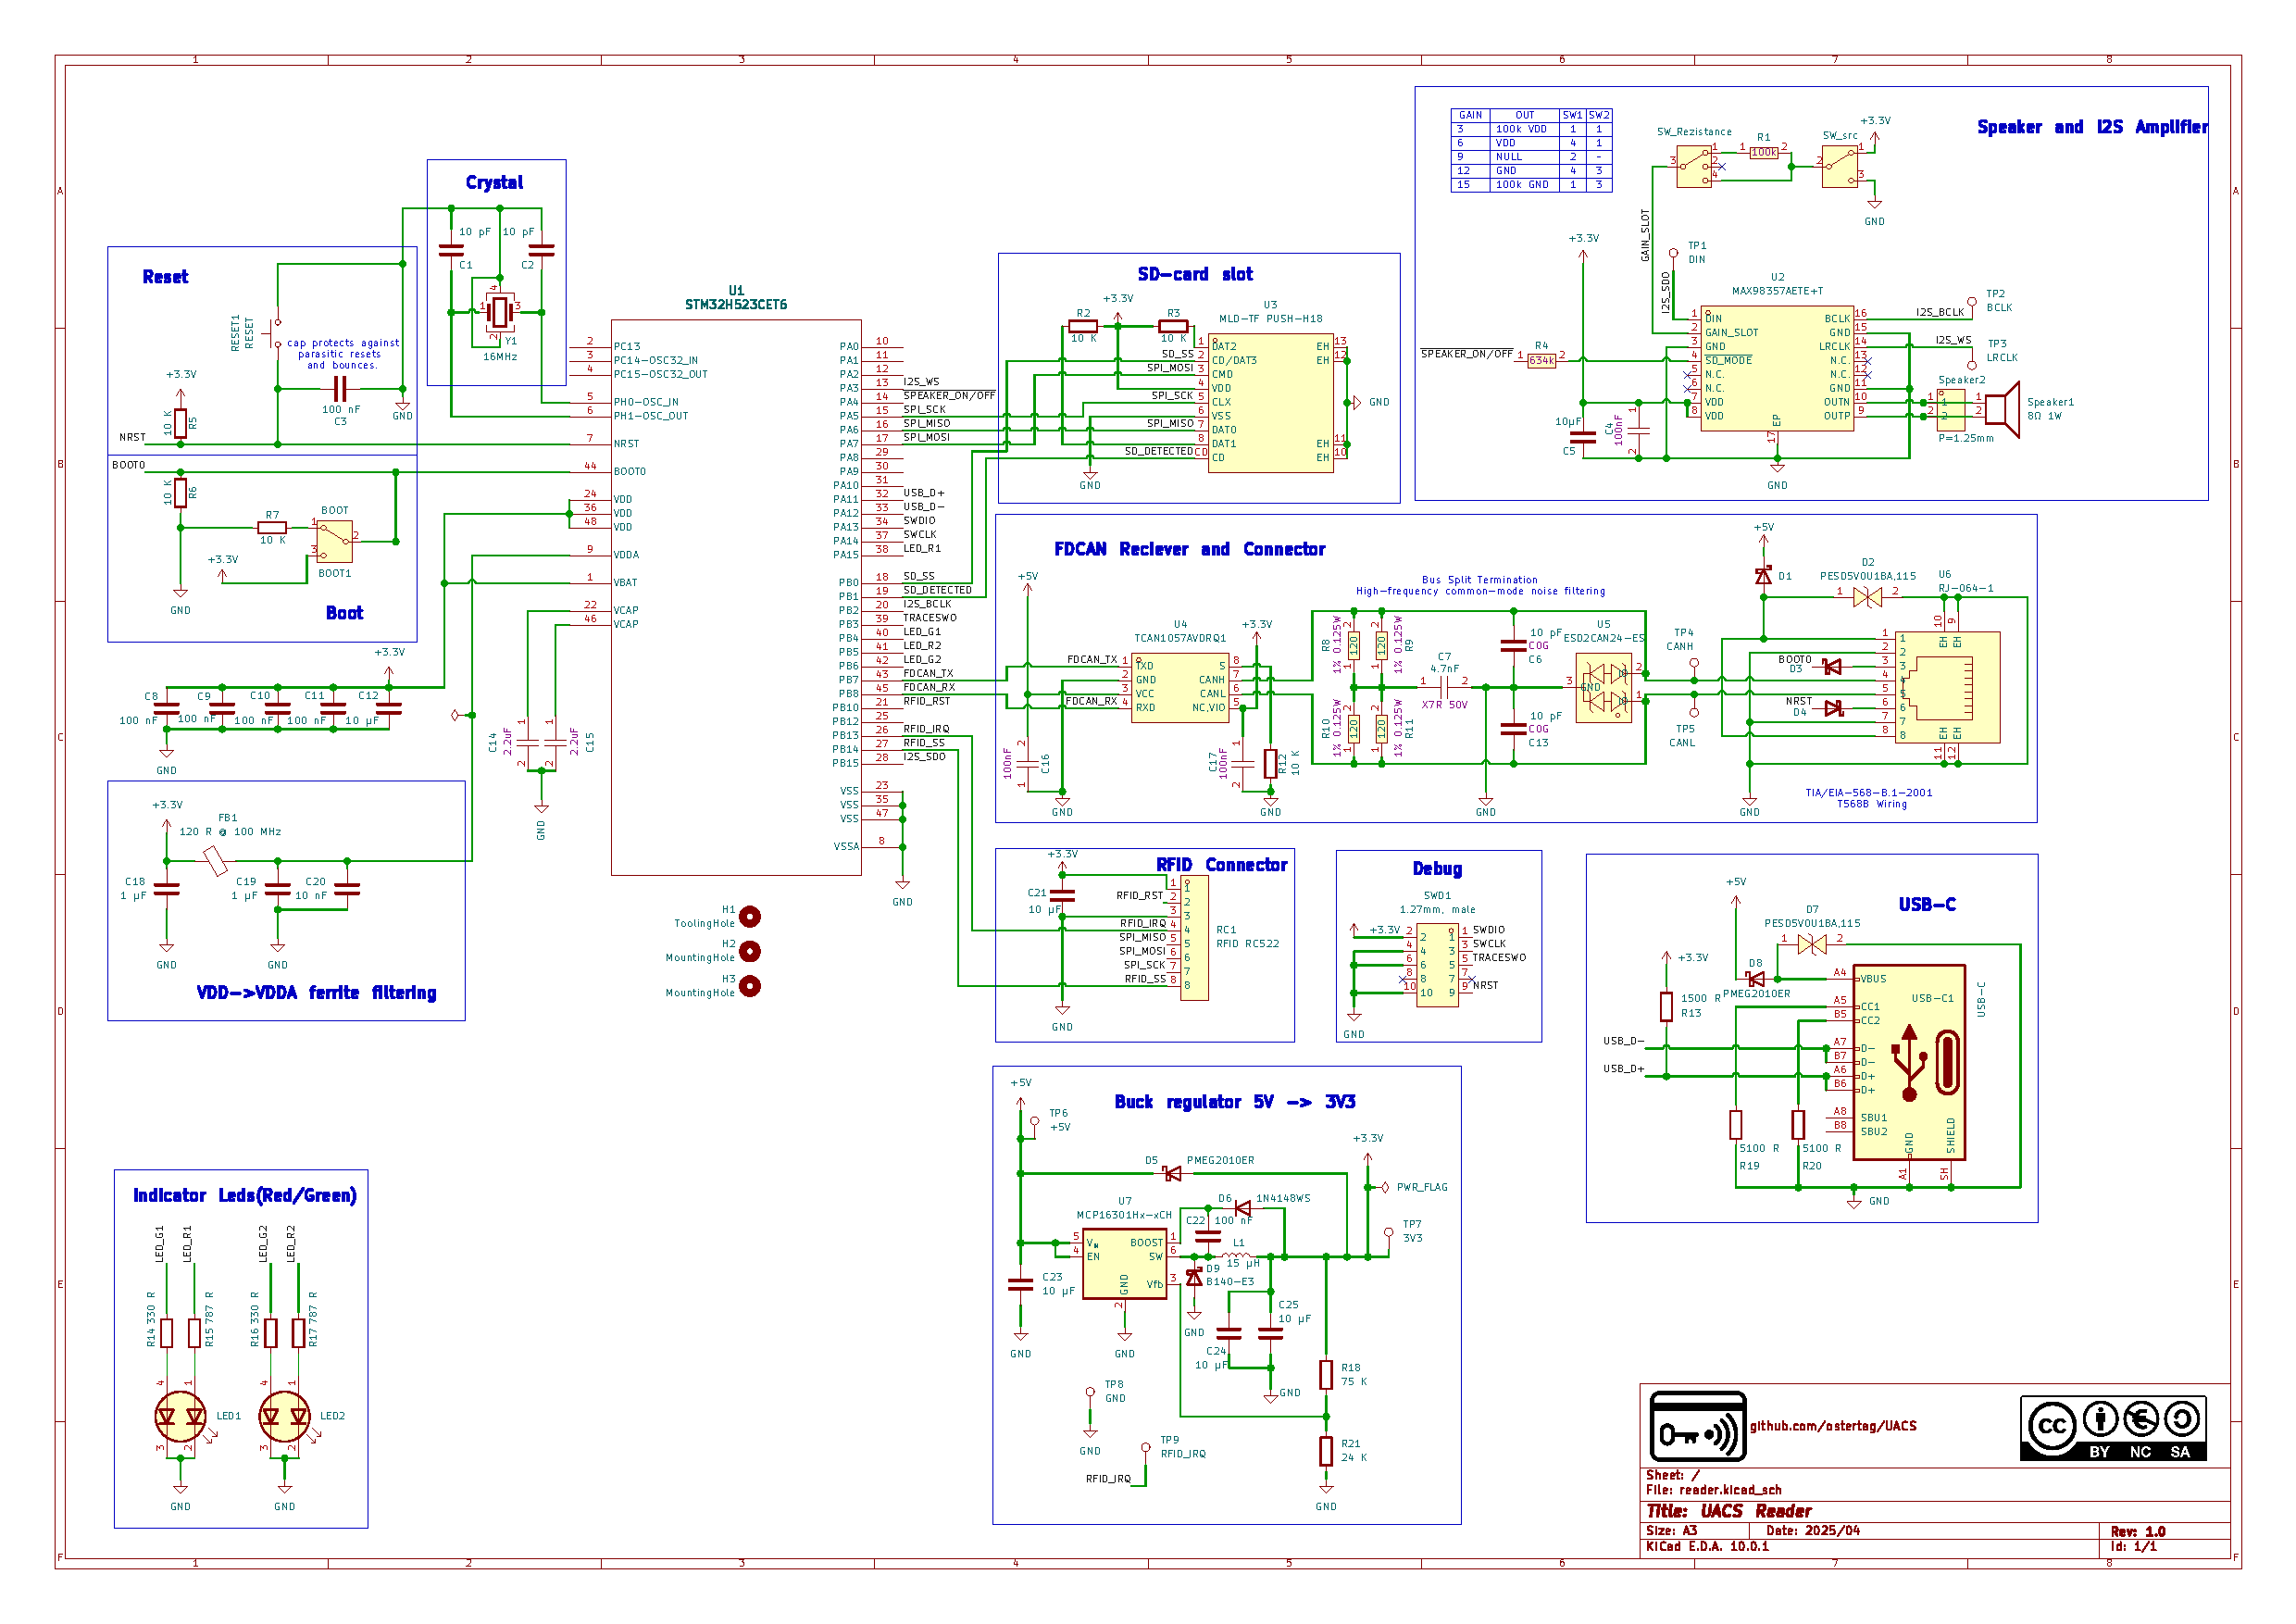
\includegraphics[width=\textheight, height=\textwidth, keepaspectratio]{images/schematic.pdf}}
  \caption{UACS board full schematic.}
  \label{obr:schematic}
\end{figure}

% ================================================================
\section{Microcontroller --- STM32H523CET6}
\label{sec:mcu}
% ================================================================

The STM32H523CET6 is the central controller of the board. It is supplied in an LQFP-48
package and runs the Cortex-M33 core at \SI{250}{\mega\hertz}~\cite{ref1}. All peripheral
communication --- SPI, I\textsuperscript{2}S, FDCAN, and USB --- is handled by this
device.

% ----------------------------------------------------------------
\subsection{Debug Interface (SWD)}
\label{subsec:swd}
% ----------------------------------------------------------------

The board exposes a 10-pin 1.27\,mm-pitch Cortex debug connector (SWD1), driven by an
STLINK-V3PWR probe.

The STM32H523 supports both JTAG and Serial Wire Debug (SWD), as well as the Embedded
Trace Macrocell (ETM)~\cite{ref1}. SWD was selected over JTAG because it reduces the
debug interface to two active signals --- SWDIO and SWCLK --- while providing equivalent
core-debug and memory-access capability to the higher-pin-count JTAG
interface~\cite{ref12,ref13}. On a pin-constrained LQFP-48 device, freeing the JTAG pins
(TDI, TDO, nTRST) for other functions is a meaningful saving, and SWD is the conventional
default for Cortex-M bring-up~\cite{ref13}.

The Serial Wire Output trace pin (TRACESWO) is brought out on PB3, enabling single-wire
instrumentation trace (printf-style debug output) without consuming a UART peripheral.
The connector follows the standard 10-pin 1.27\,mm Cortex-debug pinout, which balances
size against reliability~\cite{ref13}.

The STLINK-V3PWR probe was already available and was therefore the natural choice. In
addition to SWD/SWV (supported up to \SI{10}{\mega\hertz}) it integrates a source
measurement unit~(SMU) with a programmable 1.6--\SI{3.6}{\volt} output and current
measurement from the nanoampere range up to \SI{500}{\milli\ampere}~\cite{ref4}. This
capability is useful during development for verifying the board's power budget, since the
entire \SI{3.3}{\volt} system is supplied by a single \SI{1}{\ampere} regulator. The
probe is supported directly by the STM32CubeMonitor-Power software tool~\cite{ref4}.

% ----------------------------------------------------------------
\subsection{Reset Circuit}
\label{subsec:reset}
% ----------------------------------------------------------------

The NRST line is shared between three reset sources: the on-board push button (RESET1),
the remote reset line carried over the RJ45 connector
(Section~\ref{subsec:rj45}), and the STLINK debug probe. Tying the probe's reset into the
same net improves recovery when firmware or a low-power state would otherwise block a
debug attach~\cite{ref13}.

\paragraph{Resistor R5.}
A \SI{10}{\kilo\ohm} pull-up resistor holds the NRST line high during normal operation.
Without it the line would float and could trigger spurious resets from noise.

\paragraph{Capacitor C3.}
A \SI{100}{\nano\farad} capacitor from NRST to GND provides debounce for the mechanical
reset button and protection against parasitic resets. ST explicitly recommends an external
capacitor on NRST for exactly this purpose~\cite{ref1}.

% ----------------------------------------------------------------
\subsection{BOOT0 Circuit}
\label{subsec:boot0}
% ----------------------------------------------------------------

BOOT0 selects whether the MCU starts from user flash (normal operation) or from the
embedded system bootloader. The STM32H523 embedded bootloader, located in system memory
and programmed by ST during production, can reprogram the flash over USART, I\textsuperscript{2}C,
I\textsuperscript{3}C, SPI, FDCAN, or USB-FS (via DFU)~\cite{ref1}. On UACS, USB-FS DFU
is the relevant path (Section~\ref{sec:usb}).

BOOT0 is additionally exposed on the RJ45 connector
(Section~\ref{subsec:rj45}), so the bootloader can be entered remotely without physical
access to the board.

\paragraph{Resistor R6.}
A \SI{10}{\kilo\ohm} pull-down resistor holds BOOT0 low during normal operation. With
BOOT0 low, the device boots from user flash at address \texttt{0x0800\,0000}~\cite{ref1}.

\paragraph{Resistor R7.}
A \SI{10}{\kilo\ohm} series resistor is placed between the R6 junction and the BOOT1
switch to limit current and provide isolation between the pull-down and the switch.

\paragraph{Switch BOOT1.}
An SPDT switch that selects GND (normal boot) or \SI{3.3}{\volt} (bootloader entry).
Connecting BOOT0 to \SI{3.3}{\volt} causes the MCU to enter the embedded system
bootloader on the next reset.

% ----------------------------------------------------------------
\subsection{Crystal Oscillator}
\label{subsec:crystal}
% ----------------------------------------------------------------

A \SI{16}{\mega\hertz} crystal (Y1, SMD3225-4P, 10\,pF load) provides the high-speed
external (HSE) clock. The STM32H523 supports a 4--\SI{50}{\mega\hertz} HSE
oscillator~\cite{ref1}. Although the device has an internal \SI{64}{\mega\hertz} HSI
oscillator, an external crystal is used because the USB and CAN peripherals require a
more accurate and stable time base than the internal RC oscillator can guarantee. The USB
full-speed interface has particularly tight frequency-tolerance requirements.

No 32.768\,kHz crystal is fitted; the LSE pins (PC14/PC15) are left unconnected and
configured in Analog mode.

\paragraph{Capacitors C1 and C2.}
Two \SI{10}{\pico\farad} C0G load capacitors are placed to GND, one on each side of the
crystal, matched to its specified 10\,pF load capacitance. C0G (Class~1) dielectric is
used because its capacitance is essentially independent of temperature and applied
voltage --- typically within $\pm30$\,ppm/°C --- which is important for a stable
oscillator load~\cite{ref19,ref20}.

% ----------------------------------------------------------------
\subsection{VCAP --- Internal Regulator Capacitors}
\label{subsec:vcap}
% ----------------------------------------------------------------

The STM32H5 family integrates an LDO voltage regulator (nominally
\SI{3.3}{\volt}~$\rightarrow$~\SI{1.2}{\volt} core) that requires external stabilisation
capacitors on its VCAP pin(s)~\cite{ref1}. The datasheet specifies this requirement
explicitly in Section~5.3.2, ``VCAP external capacitor''~\cite{ref1}.

\paragraph{Capacitors C14 and C15.}
Two \SI{2.2}{\micro\farad} capacitors, one per VCAP pin, are placed to GND. These are
mandated by the datasheet for the internal regulator's stability and are not
interchangeable with generic decoupling --- the value and placement are part of the
regulator's stability requirement.

% ----------------------------------------------------------------
\subsection{Power Pins and Decoupling}
\label{subsec:mcu-power}
% ----------------------------------------------------------------

The STM32H523 uses several supply domains: the main VDD digital supply, an analog supply
(VDDA), a USB supply domain, and the VBAT backup domain~\cite{ref1}.

\begin{itemize}
  \item \textbf{VDD} --- supplied from +\SI{3.3}{\volt}; decoupled with C8--C11
        (\SI{100}{\nano\farad} each) for high-frequency bypass, plus C12
        (\SI{10}{\micro\farad}) for bulk capacitance.
  \item \textbf{VDDA} --- analog supply, filtered from the \SI{3.3}{\volt} rail through
        the VDDA filter (Section~\ref{subsec:vdda}).
  \item \textbf{VBAT} --- tied to the \SI{3.3}{\volt} rail, since no backup battery is
        used.
  \item \textbf{VSS / VSSA} --- ground.
\end{itemize}

% ----------------------------------------------------------------
\subsection{RFID Reader --- RC522 Module (MFRC522)}
\label{subsec:rfid}
% ----------------------------------------------------------------

The RFID front end is an RC522 module based on the NXP MFRC522 IC, mounted on an 8-pin
2.54\,mm socket (RC1) and connected to the MCU over SPI.

The RC522 module was selected because it was used in the predecessor project, allowing
existing experience and firmware to be carried over. The MFRC522 is a 13.56\,MHz
reader/writer IC supporting the ISO/IEC~14443~A\,/\,MIFARE protocol family --- MIFARE
Mini, 1K, 4K, Ultralight, DESFire~EV1, MIFARE Plus, and NTAG --- with a host SPI
interface running up to 10\,Mbit/s~\cite{ref3}.

\textbf{Interface signals:}
\begin{itemize}
  \item \textbf{SPI} --- shares SPI1 with the SD card (Section~\ref{sec:sdcard}); chip
        select is software-controlled on PB14 (RFID\_SS), active low.
  \item \textbf{RST (PB10)} --- the MCU drives the module's NRSTPD pin as a push-pull
        output. The pin defaults high at boot so the reader starts in normal operation;
        driving it low triggers a hard reset/power-down of the module~\cite{ref3}.
  \item \textbf{IRQ (PB13)} --- the module's interrupt output drives EXTI13, configured
        for falling-edge interrupts, enabling interrupt-driven card detection rather than
        polling.
\end{itemize}

On the MFRC522, the IRQ pin is open-drain and active-low by default~\cite{ref3}, which
matches the MCU's falling-edge EXTI configuration; only an MCU-side internal pull-up is
required on PB13, with no external resistor. The MFRC522's CommIEnReg register must be
configured in firmware to enable interrupt propagation to the IRQ pin~\cite{ref3}.

\paragraph{Capacitor C21.}
A \SI{10}{\micro\farad} local bypass capacitor is placed on the module VCC pin. VCC
connects directly to the \SI{3.3}{\volt} rail. (PB12 is left unconnected; an earlier plan
to use it for switched module power was dropped, since a single GPIO cannot source the
MFRC522's worst-case current.)

% ================================================================
\section{SD Card --- MLD-TF PUSH-H18}
\label{sec:sdcard}
% ================================================================

The micro-SD slot (U3) stores the audio files played back through the amplifier.

The preferred interface would have been the dedicated SDMMC peripheral, which provides
higher throughput than SPI. However, the SDMMC peripheral on the STM32H523 is only
available on larger packages; on the LQFP-48 the required pins are not bonded out, so
SDMMC is physically unavailable and SPI is the only option~\cite{ref1}. This is a package
constraint, not a design preference.

The SD card shares SPI1 with the RC522 reader, with its own software chip select on PB0
(SD\_SS). In SPI mode, the card's CD/DAT3 pin (slot pin~2) functions as the active-low
chip select; this is confirmed by the slot's pin table, which labels pin~2 as CD/DAT3
with I/O type~PP~\cite{ref8}.

The MLD-TF PUSH-H18 uses a push-push ejection mechanism (card ejects on the second
press); the card-detect switch is a separate mechanical contact from the signal
pins~\cite{ref8}.

\paragraph{Card Detect --- PB1.}
The slot's dedicated card-detect mechanical contact drives PB1 (SD\_DETECTED) as a GPIO
input, allowing the firmware to detect card insertion and removal.

\paragraph{Resistors R2 and R3.}
Two \SI{10}{\kilo\ohm} pull-up resistors are placed to \SI{3.3}{\volt} on the DAT1
line~(R2) and the DAT2 line~(R3). In SPI mode both of these data lines are unused; the
pull-ups keep them at a defined high level rather than floating.

% ================================================================
\section{Power Supply}
\label{sec:power}
% ================================================================

\subsection{Architecture}
\label{subsec:power-arch}

The board accepts power from two independent \SI{5}{\volt} sources, diode-OR-ed onto a
common +\SI{5}{\volt} rail and then stepped down to \SI{3.3}{\volt} by a buck converter.

\begin{table}[htbp]
  \centering
  \caption{Power input OR-ing and ESD protection.}
  \label{tab:power-inputs}
  \begin{tabular}{lll}
    \toprule
    Source       & OR-ing diode       & ESD protection           \\
    \midrule
    USB-C VBUS   & D8 (PMEG2010ER)    & D7 (PESD5V0U1BA,115)     \\
    RJ45 pair (brown) & D1 (PMEG2010ER) & D2 (PESD5V0U1BA,115)  \\
    \bottomrule
  \end{tabular}
\end{table}

The two inputs serve different operational scenarios. The RJ45 input is the primary supply
during normal deployment, where the board is powered from the CAN cabling
infrastructure. The USB-C input is used during development and programming, when the board
is connected to a PC without the full CAN harness. Diode OR-ing lets both sources be
connected simultaneously without back-feeding. Each TVS diode is placed as close as
possible to its respective input connector for effective clamping~\cite{ref10}.

% ----------------------------------------------------------------
\subsection{Buck Converter --- MCP16301H}
\label{subsec:buck}
% ----------------------------------------------------------------

The MCP16301H (U7) is a high-voltage-input, integrated-switch, fixed-frequency step-down
converter in a SOT-23-6 package~\cite{ref2}. It is AEC-Q100 Grade~1
automotive-qualified and can supply up to \SI{1}{\ampere} at \SI{3.3}{\volt}
output~\cite{ref2}. The part was carried over from the previous version of the design,
where it was already proven.

The UACS buck stage follows the MCP16301H datasheet's own \SI{3.3}{\volt} reference
design very closely, which is a deliberate choice for a known-good result.

\paragraph{Inductor L1.}
A \SI{15}{\micro\henry} inductor is used. The datasheet explicitly recommends
\SI{15}{\micro\henry} for a \SI{3.3}{\volt} output, derived from the inductor-selection
constant~$K$:

\begin{equation}
  K = \frac{V_\mathrm{OUT}}{L}
  \label{eq:buck-k}
\end{equation}

where $K$ should equal \SI{0.22}{\volt\per\micro\henry}, giving:

\begin{equation}
  L = \frac{V_\mathrm{OUT}}{K} = \frac{3.3}{0.22} \approx \SI{15}{\micro\henry}
  \label{eq:buck-L}
\end{equation}

\begin{table}[htbp]
  \centering
  \caption{MCP16301H inductor selection for common output voltages~\cite{ref2}.}
  \label{tab:inductor}
  \begin{tabular}{S[table-format=2.1]S[table-format=1.2]l}
    \toprule
    {$V_\mathrm{OUT}$ (V)} & {$K$ (V/\textmu H)} & {Standard $L$} \\
    \midrule
    2.0  & 0.20 & \SI{10}{\micro\henry}  \\
    3.3  & 0.22 & \SI{15}{\micro\henry}  \\
    5.0  & 0.23 & \SI{22}{\micro\henry}  \\
    12.0 & 0.21 & \SI{56}{\micro\henry}  \\
    15.0 & 0.22 & \SI{68}{\micro\henry}  \\
    \bottomrule
  \end{tabular}
\end{table}

\paragraph{Diode D9 (B140-E3, SMA).}
Schottky freewheeling diode; the datasheet reference design uses the B140~\cite{ref2}.

\paragraph{Diode D6 (1N4148WS).}
Boost (bootstrap) diode. The datasheet specifically recommends a 1N4148 for this role for
its fast recovery speed, voltage blocking capability, wide availability, and low
cost~\cite{ref2}.

\paragraph{Capacitor C22.}
A \SI{100}{\nano\farad} boost capacitor. The datasheet recommends a \SI{0.1}{\micro\farad}
X5R/X7R capacitor for all applications~\cite{ref2}.

\paragraph{Capacitors C23, C24, C25.}
C23 (\SI{10}{\micro\farad}) is the input capacitor; C24 and C25
(\SI{10}{\micro\farad} each) are output capacitors placed in parallel. Their values are
consistent with the datasheet's recommended input/output capacitance~\cite{ref2}.

\paragraph{Diode D5 (PMEG2010ER).}
Back-powering protection diode between the \SI{3.3}{\volt} output and the \SI{5}{\volt}
input, reverse-biased during normal operation. It prevents the \SI{3.3}{\volt} rail from
back-feeding the \SI{5}{\volt} input when only the \SI{3.3}{\volt} side is powered ---
for example, when supplied from the STLINK probe during development.

\paragraph{Feedback Divider (R18 and R21) --- Output Voltage Setting.}
The MCP16301H regulates to an internal feedback reference of \textbf{0.800\,V (typical)}.
The output voltage is set by an external resistor divider according to the datasheet
formula~\cite{ref2}:

\begin{equation}
  R_\mathrm{TOP} = R_\mathrm{BOT} \times \left(\frac{V_\mathrm{OUT}}{V_\mathrm{FB}} - 1\right)
  \label{eq:feedback-rtop}
\end{equation}

equivalently:

\begin{equation}
  V_\mathrm{OUT} = V_\mathrm{FB} \times \left(1 + \frac{R_\mathrm{TOP}}{R_\mathrm{BOT}}\right)
  \label{eq:feedback-vout}
\end{equation}

With the values used on UACS ($R_{18} = \SI{75}{\kilo\ohm} = R_\mathrm{TOP}$,
$R_{21} = \SI{24}{\kilo\ohm} = R_\mathrm{BOT}$):

\begin{equation}
  V_\mathrm{OUT} = 0.800 \times \left(1 + \frac{75}{24}\right) = 0.800 \times 4.125 \approx \SI{3.30}{\volt} \quad \checkmark
  \label{eq:vout-calc}
\end{equation}

The datasheet's own example \SI{3.3}{\volt} divider uses $R_\mathrm{TOP} = \SI{31.6}{\kilo\ohm}$
and $R_\mathrm{BOT} = \SI{10}{\kilo\ohm}$~\cite{ref2}. UACS uses higher-value resistors
(\SI{75}{\kilo\ohm} / \SI{24}{\kilo\ohm}); both ratios produce \SI{3.3}{\volt}. The higher
values were carried over from the predecessor design, where they were chosen to reduce
quiescent current through the divider.

% ----------------------------------------------------------------
\subsection{VDDA Filter}
\label{subsec:vdda}
% ----------------------------------------------------------------

The MCU analog supply (VDDA) is filtered from the digital \SI{3.3}{\volt} rail to keep
switching noise out of the analog domain (ADC reference, internal oscillator). A ferrite
bead in series with the supply, combined with decoupling capacitors on each side, forms a
low-pass filter that absorbs high-frequency noise and dissipates it as heat; this is the
standard technique for isolating a sensitive analog supply from a noisier digital
rail~\cite{ref21}.

\paragraph{Ferrite Bead FB1.}
A \SI{120}{\ohm} @ \SI{100}{\mega\hertz}, \SI{500}{\milli\ampere}, 0603 ferrite bead acts
as the series filter element, presenting high impedance to high-frequency noise while
passing DC with negligible voltage drop.

\paragraph{Capacitor C18.}
A \SI{1}{\micro\farad} capacitor placed before the ferrite bead, from the digital
\SI{3.3}{\volt} rail to GND. Together with the bead, it forms the input side of the
low-pass filter.

\paragraph{Capacitors C19 and C20.}
A \SI{1}{\micro\farad} and a \SI{10}{\nano\farad} capacitor placed after the ferrite
bead, from the VDDA node to GND. The combination of C19 and C20 provides filtering across
a wide frequency range, covering both mid-frequency and high-frequency noise at the
filtered VDDA node.

% ================================================================
\section{CAN Bus --- TCAN1057A}
\label{sec:can}
% ================================================================

The CAN interface links the board to the host Raspberry Pi. The transceiver is the
TCAN1057AVDRQ1 (U4), an automotive-grade CAN~FD device in a SOIC-8 package, driven by
the MCU FDCAN1 peripheral (PB7~TX, PB8~RX)~\cite{ref7}.

The TCAN1057A was selected because it meets the required parameters, including CAN~FD
support. CAN~FD (Flexible Data-rate) extends classical CAN by allowing the data phase to
be transmitted at a higher bit rate than the arbitration phase, and by increasing the
maximum payload from 8 to 64 bytes per frame~\cite{ref14,ref15}. In practice CAN~FD
data-phase rates of up to 5\,Mbit/s are common~\cite{ref15}, giving the link more
bandwidth and headroom than classical CAN, while remaining compatible with the familiar
CAN arbitration and error-handling mechanisms~\cite{ref14}.

% ----------------------------------------------------------------
\subsection{Transceiver Configuration}
\label{subsec:can-config}
% ----------------------------------------------------------------

\paragraph{Capacitors C16 and C17.}
Two \SI{100}{\nano\farad} bypass capacitors are placed on the transceiver VCC and GND
pins for high-frequency supply decoupling.

\paragraph{Resistor R12 --- Mode Select Pin.}
A \SI{10}{\kilo\ohm} resistor ties the S (mode-select) pin permanently to GND, placing
the transceiver in Normal Mode. The datasheet (Table~8-4) confirms: S = Low $\rightarrow$
Normal Mode (driver and receiver both enabled); S = High $\rightarrow$ Silent Mode
(driver disabled, receive-only). The datasheet explicitly states that when normal mode is
the only intended operating mode, the S pin may be tied directly to GND via a pull-down
resistor~\cite{ref7}.

% ----------------------------------------------------------------
\subsection{RJ45 Cabling and Pair Assignment}
\label{subsec:rj45}
% ----------------------------------------------------------------

The bus is carried over standard RJ45/Cat5 cabling. The eight conductors are assigned as
four pairs:

\begin{table}[htbp]
  \centering
  \caption{RJ45 connector pair assignments.}
  \label{tab:rj45}
  \begin{tabular}{ll}
    \toprule
    Connector pins & Pair function \\
    \midrule
    1 + 2 & GND / +\SI{5}{\volt} (power) \\
    3 + 6 & BOOT0 / NRST (remote MCU control) \\
    4 + 5 & CANH / CANL (differential bus) \\
    7 + 8 & GND / +\SI{5}{\volt} (power) \\
    \bottomrule
  \end{tabular}
\end{table}

In a Cat5 cable, pins~4 and~5 form the centre, tightest-twisted pair. The differential
CAN signal is assigned to this pair because tight twisting maximises noise rejection:
both conductors pick up external interference almost equally as common-mode, which the
differential receiver then rejects.

Carrying BOOT0 and NRST over the cable allows remote firmware flashing and reset without
physical access to the deployed board.

\paragraph{Diodes D3 and D4 (PMEG2010ER).}
Protection diodes placed on the BOOT0~(D3) and NRST~(D4) lines respectively, guarding
against overvoltage transients on these control signals.

% ----------------------------------------------------------------
\subsection{Bus Termination}
\label{subsec:can-term}
% ----------------------------------------------------------------

Termination is the most involved part of the CAN design and is documented in full below.

\textbf{Why termination is required.} A CAN bus is a transmission line whose
characteristic impedance ($\approx$\SI{120}{\ohm} for twisted-pair CAN cable) must be
matched at both ends. Without \SI{120}{\ohm} termination at each end, signal edges reflect
from the unterminated ends and corrupt communication. Terminating both ends absorbs the
signal energy and prevents these reflections~\cite{ref16}.

\textbf{Why split termination instead of a single \SI{120}{\ohm} resistor.} In a
split-termination scheme the single \SI{120}{\ohm} resistor is replaced by two
\SI{60}{\ohm} resistors in series, with a capacitor from their midpoint to ground. The
differential impedance remains \SI{120}{\ohm} (\SI{60}{\ohm} + \SI{60}{\ohm}), so CAN
signalling is unaffected, while the midpoint capacitor provides a low-impedance path to
ground for high-frequency common-mode noise --- improving electromagnetic compatibility
(EMC)~\cite{ref17,ref18}. This is particularly valuable on a board that also carries a
switching regulator and a multi-metre cable run.

\textbf{Why two \SI{120}{\ohm} resistors in parallel per side.} Each \SI{60}{\ohm} half
is implemented using two \SI{120}{\ohm} resistors in parallel, rather than a single
\SI{60}{\ohm} part. Single \SI{60}{\ohm} resistors in the 0805 footprint are less
commonly stocked and more expensive; \SI{120}{\ohm} is a very common value, and two in
parallel give exactly \SI{60}{\ohm}. A secondary benefit is that power dissipation is
split across two resistors, halving the dissipation each must handle.

\paragraph{Resistors R8\,$\parallel$\,R9 (CANH side).}
Two \SI{120}{\ohm} resistors in parallel, giving \SI{60}{\ohm}, placed in series on CANH.
Each resistor is 0805, 1\%, \SI{0.125}{\watt}.

\paragraph{Resistors R10\,$\parallel$\,R11 (CANL side).}
Two \SI{120}{\ohm} resistors in parallel, giving \SI{60}{\ohm}, placed in series on CANL.
Same specification as R8/R9.

\paragraph{Capacitor C7.}
A \SI{4.7}{\nano\farad} X7R, \SI{50}{\volt} capacitor from the split-termination midpoint
to GND. The chosen value sits within the commonly recommended 4.7--\SI{10}{\nano\farad}
range for common-mode filtering~\cite{ref17}.

% ----------------------------------------------------------------
\subsection{High-Frequency Bypass and ESD Protection}
\label{subsec:can-hf}
% ----------------------------------------------------------------

\paragraph{Capacitors C6 and C13.}
Two \SI{10}{\pico\farad} C0G, \SI{50}{\volt} capacitors are placed from CANH~(C6) and
CANL~(C13) respectively to GND, providing additional high-frequency bypass on the bus
lines. C0G (Class~1) dielectric is specified deliberately: its capacitance is stable with
voltage and temperature, whereas a Class~2 dielectric such as X7R varies with both and
would risk rounding the fast CAN~FD signal edges~\cite{ref19,ref20}.

\paragraph{U5 --- ESD Protection (ESD2CAN24-ES, SOT-23-3).}
A CAN-specific TVS/ESD protection device placed on the bus side of the filtering network.
The device is rated for $\pm$30\,kV IEC~61000-4-2 contact and air discharge, with a
\SI{24}{\volt} reverse standoff voltage and a typical junction capacitance of 18\,pF,
making it well-suited for a CAN~FD bus~\cite{ref11}.

% ================================================================
\section{Audio Amplifier --- MAX98357A}
\label{sec:audio}
% ================================================================

The MAX98357A (U2) is a digital-input Class~D audio amplifier in a TQFN-16 package,
supplied from \SI{3.3}{\volt}. It receives audio over I\textsuperscript{2}S and drives
the loudspeaker directly.

The MAX98357A was selected for several reasons: it integrates an I\textsuperscript{2}S
receiver and a Class~D amplifier in a single device, eliminating the separate
DAC/translator, amplifier, and output-filter stages that a discrete audio path would
require; it drives the speaker directly with no external output filter; it provides
hardware-selectable gain; and it comes from a reputable manufacturer with thorough
documentation~\cite{ref6}.

The amplifier connects to the MCU I\textsuperscript{2}S peripheral over three lines:

\begin{itemize}
  \item \textbf{DIN --- PB15 (I2S\_SDO)} --- serial audio data
  \item \textbf{BCLK --- PB2 (I2S\_BCLK)} --- bit clock
  \item \textbf{LRCLK --- PA3 (I2S\_WS)} --- word select / left-right clock
\end{itemize}

The exposed pad (EP) is tied to GND. The speaker connects through a Molex 1.25\,mm
right-angle connector (Speaker2).

% ----------------------------------------------------------------
\subsection{SD\_MODE / Shutdown Control}
\label{subsec:sdmode}
% ----------------------------------------------------------------

The SD\_MODE pin controls both shutdown and the output channel mode. It is driven from
PA4 (SPEAKER\_ON/OFF) as a push-pull output. PA4 defaults low at boot, so the amplifier
starts in shutdown.

\paragraph{Resistor R4 --- SD\_MODE Series Resistor.}
The output channel mode is set by the value of the resistor placed between the GPIO and
the SD\_MODE pin. Per the MAX98357A datasheet formula~\cite{ref6}:

\begin{equation}
  R = 222.2 \times V_\mathrm{DDIO} - 100 \quad [\text{result in k}\Omega]
  \label{eq:sdmode}
\end{equation}

Substituting the \SI{3.3}{\volt} supply:

\begin{equation}
  R = 222.2 \times 3.3 - 100 \approx \SI{634}{\kilo\ohm}
  \label{eq:sdmode-val}
\end{equation}

A \textbf{\SI{634}{\kilo\ohm} $\pm$1\,\%} resistor (R4) is used. With this configuration:

\begin{itemize}
  \item \textbf{GPIO HIGH (\SI{3.3}{\volt})} $\rightarrow$ SD\_MODE pulled high through
        R4, placing the amplifier in (L/2 + R/2) mono-mix mode (active).
  \item \textbf{GPIO LOW (\SI{0}{\volt})} $\rightarrow$ amplifier in shutdown / deep
        sleep.
\end{itemize}

% ----------------------------------------------------------------
\subsection{Gain Configuration (GAIN\_SLOT)}
\label{subsec:gain}
% ----------------------------------------------------------------

The amplifier gain is set by how the GAIN\_SLOT pin is connected. The
datasheet~\cite{ref6} defines five discrete settings (Table~8):

\begin{table}[htbp]
  \centering
  \caption{MAX98357A gain settings~\cite{ref6}.}
  \label{tab:gain}
  \begin{tabular}{ll}
    \toprule
    GAIN\_SLOT connection         & Gain (dB) \\
    \midrule
    \SI{100}{\kilo\ohm} to GND   & 15 \\
    Direct to GND                & 12 \\
    Unconnected                  & 9  \\
    Direct to VDD                & 6  \\
    \SI{100}{\kilo\ohm} to VDD   & 3  \\
    \bottomrule
  \end{tabular}
\end{table}

To make all five settings selectable in hardware, the board uses a two-switch network:

\begin{itemize}
  \item \textbf{SW1 (SP3T)} --- selects the path as open (NC), direct
        (\SI{0}{\ohm}), or through a \SI{100}{\kilo\ohm} resistor.
  \item \textbf{SW2 (SPDT)} --- selects whether that path connects to GND or VDD.
\end{itemize}

The default state (GAIN\_SLOT unconnected) gives \textbf{9\,dB}.

\paragraph{Resistor R1.}
A \SI{100}{\kilo\ohm} gain-setting resistor used for the 3\,dB and 15\,dB settings.
Its value is taken directly from the datasheet gain table~\cite{ref6}.

% ----------------------------------------------------------------
\subsection{Speaker and Power Budget}
\label{subsec:speaker}
% ----------------------------------------------------------------

An \textbf{\SI{8}{\ohm}, \SI{1}{\watt}} speaker is used. The output power into the
load is estimated from the supply voltage and load resistance:

\begin{equation}
  P = \frac{V_\mathrm{DD}^{2}}{2 \times R_L}
    = \frac{3.3^{2}}{2 \times 8}
    \approx \SI{0.68}{\watt}
  \label{eq:speaker-power}
\end{equation}

An \SI{8}{\ohm} load was chosen deliberately over \SI{4}{\ohm}. At \SI{4}{\ohm}, the
output power and corresponding current draw roughly double, which would push the peak
current close to the \SI{1}{\ampere} limit of the single buck regulator supplying the
whole board. The \SI{8}{\ohm} choice keeps the peak current comfortably within budget.

% ----------------------------------------------------------------
\subsection{Decoupling}
\label{subsec:audio-decoupling}
% ----------------------------------------------------------------

\paragraph{Capacitors C4 and C5.}
C4 (\SI{100}{\nano\farad}) and C5 (\SI{10}{\micro\farad}) provide supply decoupling on
the amplifier VDD pins, covering both high-frequency and bulk requirements.

% ================================================================
\section{USB-C Interface}
\label{sec:usb}
% ================================================================

The USB-C interface (USB-C1) is a 14-pin horizontal SMD Type-C receptacle used to connect
the board to a PC.

The interface is USB~2.0 only --- carried over from the previous version; there is no
requirement for higher transfer rates in this application. The board operates purely as a
USB device (USB\_DRD\_FS), used for firmware flashing (USB-FS DFU) and debugging; it does
not act as a host. The STM32H523 provides one USB~2.0 full-speed device
interface~\cite{ref1}.

The USB~2.0 differential data pair uses pins PA11~(D+) and PA12~(D$-$).

The USB-C circuit follows the standard UFP (upstream-facing port / device) topology as
specified in the USB Type-C specification~\cite{ref22,ref23}.

\paragraph{Resistors R19 and R20.}
Two \SI{5.1}{\kilo\ohm} Rd pull-down resistors are placed on CC1 and CC2 to GND. The
USB Type-C specification requires a device (UFP) to present a \SI{5.1}{\kilo\ohm}
$\pm$10\,\% Rd pull-down on each CC pin; this is the only acceptable value for
advertising a standard Type-C current contract~\cite{ref22,ref23}. The two pins are
pulled down independently --- not tied together~\cite{ref23}.

\paragraph{Resistor R13.}
A \SI{1.5}{\kilo\ohm} resistor is placed between the \SI{3.3}{\volt} rail and VBUS for
VBUS sensing.

\paragraph{Diode D7 (PESD5V0U1BA,115).}
A bidirectional TVS diode on VBUS for ESD protection. The device provides a \SI{5}{\volt}
reverse standoff voltage, 2.9\,pF typical capacitance, and up to 10\,kV IEC~61000-4-2
protection in a SOD323 package~\cite{ref10}.

\paragraph{Diode D8 (PMEG2010ER).}
An OR-ing Schottky diode feeding VBUS into the shared +\SI{5}{\volt} power
rail~\cite{ref9}.

SBU1 and SBU2 pins are left unconnected, as they are not required for USB~2.0 device
operation. The shield and GND~(A1) are tied to GND.

% ================================================================
\section{Indicator LEDs --- APHBM2012 Series}
\label{sec:leds}
% ================================================================

The board carries two dual-colour (red + emerald-green) SMD indicator LEDs from the
Kingbright APHBM2012 series. Each LED has independent red and green elements with common
cathodes to GND, so each colour is driven through its own current-limiting resistor from
a GPIO.

\begin{table}[htbp]
  \centering
  \caption{Indicator LED assignments.}
  \label{tab:leds}
  \begin{tabular}{p{0.05\textwidth} p{0.27\textwidth} p{0.12\textwidth}
                  p{0.20\textwidth} p{0.20\textwidth}}
    \toprule
    Ref  & Part                    & Nominal current & Green signal     & Red signal       \\
    \midrule
    LED1 & APHBM2012LSURKZGKC      & \SI{2}{\milli\ampere} & LED\_G1 (PB4)  & LED\_R1 (PA15) \\
    LED2 & APHBM2012LSURKZGKC      & \SI{2}{\milli\ampere} & LED\_G2 (PB6)  & LED\_R2 (PB5)  \\
    \bottomrule
  \end{tabular}
\end{table}

The predecessor board used two different LED variants (2\,mA and 20\,mA) because the
required brightness was unknown during the initial design. Once confirmed that 2\,mA
provides sufficient visibility for the application, both LEDs were standardised to the
low-current APHBM2012LSURKZGKC variant, simplifying the BOM.

Each LED element is driven from a GPIO through a series current-limiting resistor, with
the cathode tied to GND.

\paragraph{Current-Limiting Resistors.}
The current-limiting resistor value is calculated from the supply voltage, the LED forward
voltage, and the target forward current:

\begin{equation}
  R = \frac{V_\mathrm{DD} - V_f}{I_f} \qquad \text{with } V_\mathrm{DD} = \SI{3.3}{\volt}
  \label{eq:led-r}
\end{equation}

Using the typical forward voltages from the Kingbright datasheets~\cite{ref5}.
For LED1 with $I_f = \SI{2}{\milli\ampere}$ ($V_f$: Red \SI{1.75}{\volt},
Green \SI{2.65}{\volt}):

\begin{align}
  R_\mathrm{red}   &= \frac{3.3 - 1.75}{0.002} = \SI{775}{\ohm}
                      \quad\rightarrow\quad \textbf{\SI{787}{\ohm}} \text{ chosen (R15)}
  \label{eq:r-red} \\
  R_\mathrm{green} &= \frac{3.3 - 2.65}{0.002} = \SI{325}{\ohm}
                      \quad\rightarrow\quad \textbf{\SI{330}{\ohm}} \text{ chosen (R14)}
  \label{eq:r-green}
\end{align}

Both LEDs are identical, so LED2 uses the same resistor values:
R17 = \SI{787}{\ohm} (red) and R16 = \SI{330}{\ohm} (green).
In both cases the nearest standard resistor value was selected.

\begin{figure}[p]
  \centering
  \rotatebox{-90}{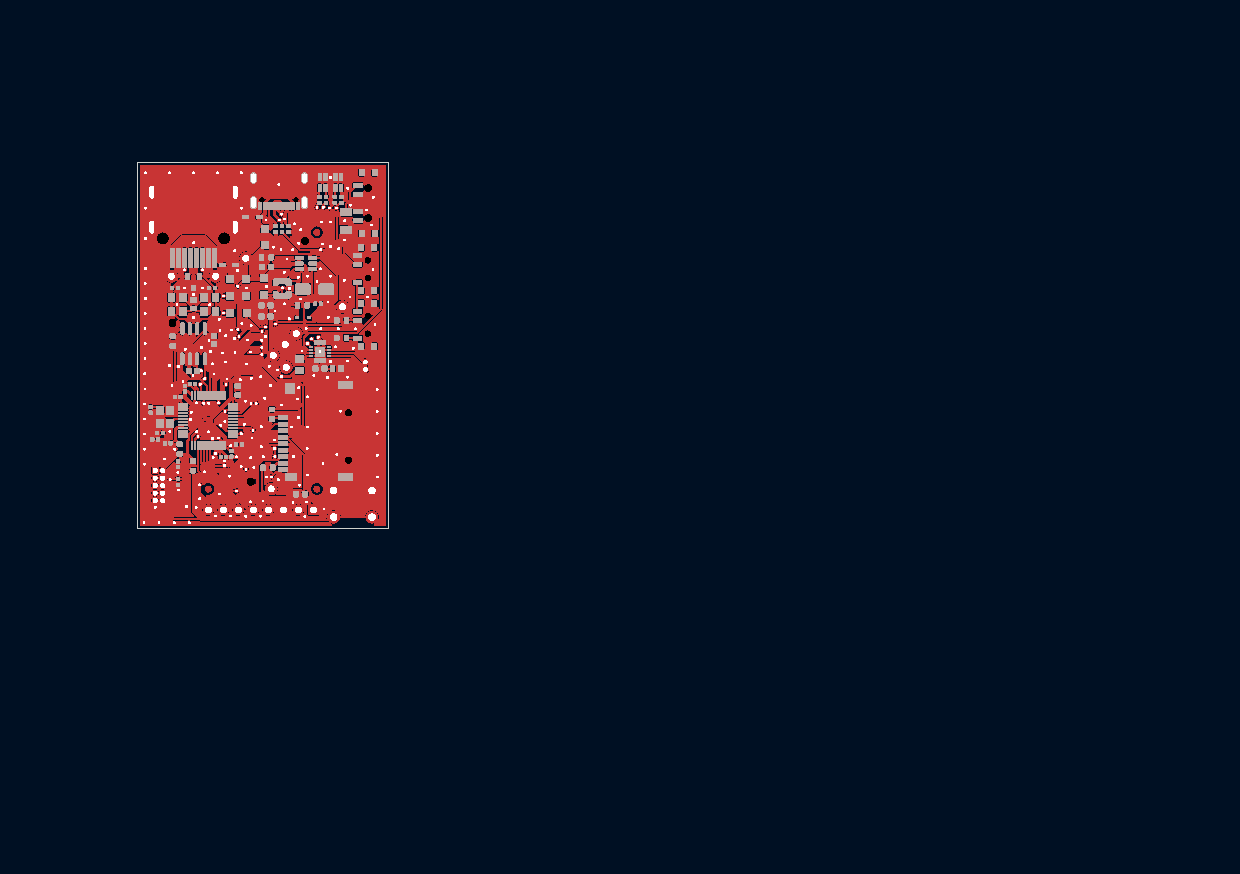
\includegraphics[width=\textheight, height=\textwidth, keepaspectratio]{images/pcb_f.pdf}}
  \caption{UACS PCB --- front copper layer (F.Cu).}
  \label{obr:pcb-front}
\end{figure}

\begin{figure}[p]
  \centering
  \rotatebox{-90}{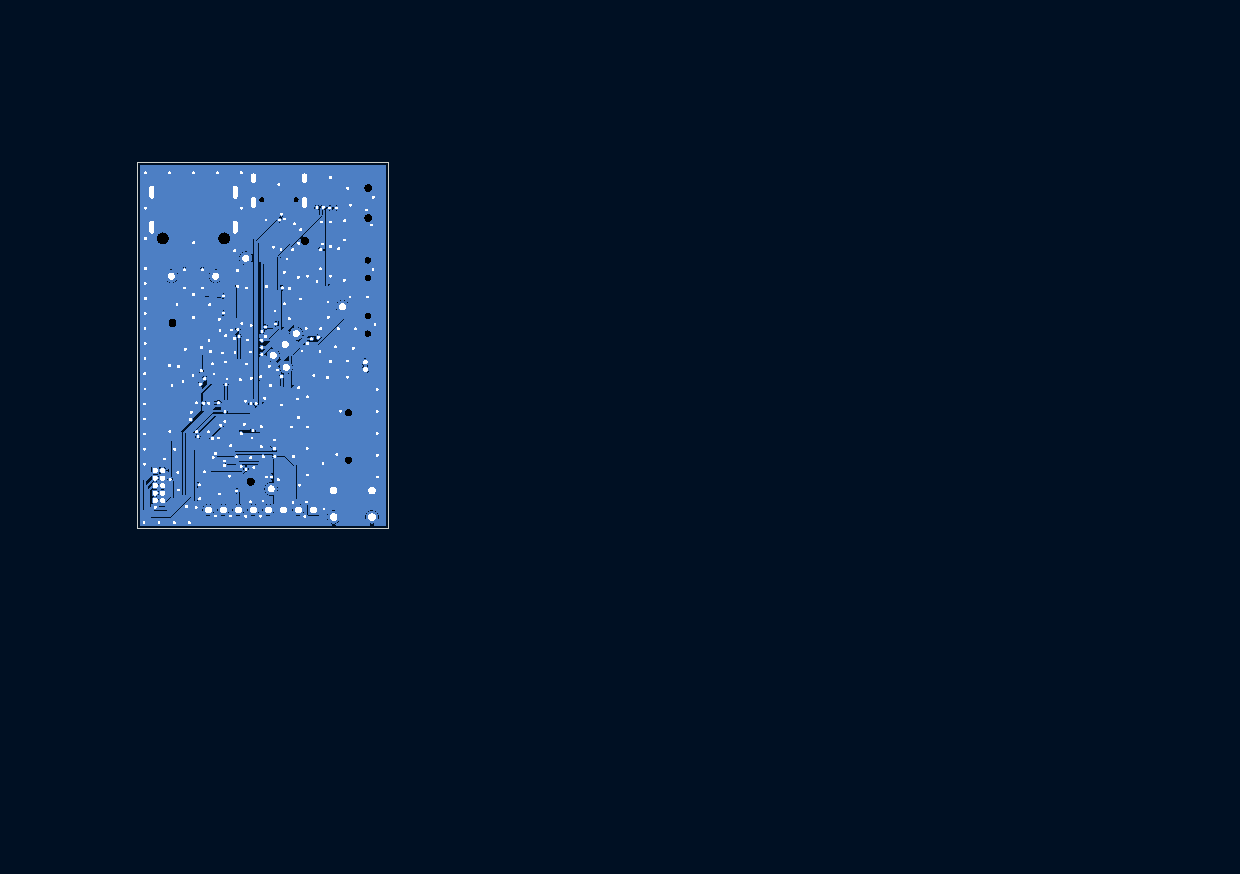
\includegraphics[width=\textheight, height=\textwidth, keepaspectratio]{images/pcb_b.pdf}}
  \caption{UACS PCB --- back copper layer (B.Cu).}
  \label{obr:pcb-back}
\end{figure}
